\documentclass[a4paper,12pt]{article}
\usepackage[T2A]{fontenc}
\usepackage[utf8]{inputenc}
\usepackage[russian]{babel}
\usepackage{amsmath,amssymb}
\usepackage{graphicx}
\usepackage{booktabs}
\usepackage{geometry}
\usepackage{float}
\usepackage{hyperref}
\geometry{left=2cm,right=2cm,top=2cm,bottom=2cm}

\begin{document}

\begin{titlepage}
    \centering
    {\scshape\Large МОСКОВСКИЙ ФИЗИКО-ТЕХНИЧЕСКИЙ ИНСТИТУТ \\
    (НАЦИОНАЛЬНЫЙ ИССЛЕДОВАТЕЛЬСКИЙ УНИВЕРСИТЕТ)\\
    Физтех-школа аэрокосмических технологий}
    \vspace{4cm}
    {\LARGE Отчет о выполнении лабораторной работы 3.7.1}
    \vspace{1cm}
    {\huge\bf Скин-эффект}
    \vfill
    \begin{flushright}
        {\LARGE Губарев Никита, Б03-502}
    \end{flushright}
    \vfill
    \today
\end{titlepage}

\tableofcontents
\newpage

\section{Аннотация}
Цель работы: исследование проникновения переменного магнитного поля в медный полый цилиндр (скин-эффект), определение проводимости материала экрана четырьмя независимыми способами.

\section{Теоретические сведения}
При помещении проводящего цилиндра в переменное магнитное поле в стенке возникает вихревое электрическое поле, которое по закону Ома создаёт токи Фуко. Эти токи, в свою очередь, порождают магнитное поле, компенсирующее внешнее. В результате переменное поле проникает в проводник лишь на глубину скин-слоя
\begin{equation}
    \delta = \sqrt{\frac{2}{\omega\sigma\mu_0}},
    \label{eq:delta}
\end{equation}
где $\sigma$~--- проводимость, $\mu_0=4\pi\cdot10^{-7}$~Гн/м. Для тонкостенного цилиндра радиуса $a$ и толщины $h\ll a$ связь между комплексными амплитудами поля снаружи $H_0$ и внутри $H_1$ даётся выражением
\begin{equation}
    H_1 = \frac{H_0}{\operatorname{ch}\alpha h + \frac{1}{2}\alpha a\operatorname{sh}(\alpha h)},
    \qquad \alpha = \frac{1+i}{\delta}.
    \label{eq:H1}
\end{equation}
В пределе низких частот ($\delta\gg h$) отношение модулей и сдвиг фаз равны
\begin{equation}
    \frac{|H_1|}{|H_0|} = \frac{1}{\sqrt{1+(\pi a h\sigma\mu_0\nu)^2}},
    \qquad \operatorname{tg}\psi = \pi a h\sigma\mu_0\nu.
    \label{eq:low}
\end{equation}
В пределе высоких частот ($\delta\ll h$)
\begin{equation}
    \frac{|H_1|}{|H_0|} = \frac{2\sqrt{2}\,\delta}{a}\,e^{-h/\delta},
    \qquad \psi = \frac{\pi}{4} + h\sqrt{\pi\nu\sigma\mu_0}.
    \label{eq:high}
\end{equation}
Индуктивность соленоида с экраном также зависит от частоты:
\begin{equation}
    \frac{L_{\max}-L}{L-L_{\min}} = (\pi a h\mu_0\sigma\nu)^2,
    \label{eq:L}
\end{equation}
где $L_{\max}$ и $L_{\min}$~--- индуктивности при низкой и высокой частотах соответственно.

\section{Экспериментальная установка и методика}
Схема установки приведена в описании. Переменное поле создаётся соленоидом, питаемым генератором АКИП--3420. Внутри соленоида расположен медный экран (труба). Измерительная катушка внутри экрана позволяет измерять ЭДС индукции $U$, пропорциональную $|H_1|\nu$. Ток в соленоиде $I$ измеряется амперметром. Отношение амплитуд полей определяется как
\begin{equation}
    \xi = \frac{U}{\nu I} = \xi_0 \frac{|H_1|}{|H_0|}.
\end{equation}
Коэффициент $\xi_0$ находится из условия $\xi\to\xi_0$ при $\nu\to0$. Сдвиг фаз $\psi$ между полями вычисляется по осциллограмме: $\Delta\varphi = (x/x_0)\pi$, $\psi = \Delta\varphi - \pi/2$. Индуктивность $L(\nu)$ измеряется RLC-метром.

Параметры установки: $a = d/2 = 22{,}5$~мм, $h = 1{,}5$~мм, $\mu_0 = 4\pi\cdot10^{-7}$~Гн/м. Характерная частота $\nu_h$, при которой $\delta=h$, равна
\[
    \nu_h = \frac{1}{\pi h^2\sigma\mu_0} \approx 2{,}25~\text{кГц}
\]
при табличной проводимости меди $\sigma=5\cdot10^7$~См/м.

\section{Результаты измерений и обработка}

\subsection{Низкочастотная зависимость $\xi(\nu)$}
В табл.~\ref{tab:xi_low} приведены данные для частот $22{,}5$--$113$~Гц. Величина $\xi = U/(\nu I)$ вычислена с учётом $I$ в амперах. Погрешности: $\delta\nu=1$~Гц, $\delta I=0{,}1$~мА, $\delta U=1$~мВ.

\begin{table}[H]
    \centering
    \caption{Низкие частоты}
    \label{tab:xi_low}
    \begin{tabular}{cccc}
        \toprule
        $\nu$, Гц & $I$, мА & $U$, В & $\xi$, В/(Гц$\cdot$А) \\
        \midrule
        22.5 & 452.5 & 0.1471 & 0.01445 \\
        23   & 451.63& 0.1499 & 0.01443 \\
        33   & 447.85& 0.2110 & 0.01428 \\
        43   & 442.90& 0.2684 & 0.01410 \\
        53   & 436.91& 0.3212 & 0.01387 \\
        63   & 430.34& 0.3690 & 0.01361 \\
        73   & 423.53& 0.4121 & 0.01333 \\
        83   & 416.63& 0.4506 & 0.01303 \\
        93   & 409.86& 0.4846 & 0.01272 \\
        103  & 403.31& 0.5146 & 0.01239 \\
        113  & 397.05& 0.5410 & 0.01206 \\
        \bottomrule
    \end{tabular}
\end{table}

На рис.~\ref{fig:xi_low} построена зависимость $1/\xi^2$ от $\nu^2$. Она линейна:
\[
    \frac{1}{\xi^2} = \frac{1}{\xi_0^2} + \left(\frac{\pi a h\sigma\mu_0}{\xi_0}\right)^2 \nu^2.
\]
Из графика найдены наклон $K$ и свободный член $b=1/\xi_0^2$. Тогда
\[
    \xi_0 = b^{-1/2},\qquad
    \sigma = \frac{\sqrt{K/b}}{\pi a h\mu_0}.
\]
Получено: $K = (1{,}02\pm0{,}04)\cdot10^{-6}$~В$^2$/(Гц$^2\cdot$А$^2$), $b = (4{,}78\pm0{,}02)\cdot10^{3}$~А$^2$/(В$^2$/Гц$^2$). Отсюда $\xi_0 = (1{,}446\pm0{,}003)\cdot10^{-2}$~В/(Гц$\cdot$А), $\sigma_1 = (4{,}8\pm0{,}3)\cdot10^7$~См/м.

\begin{figure}[H]
    \centering
    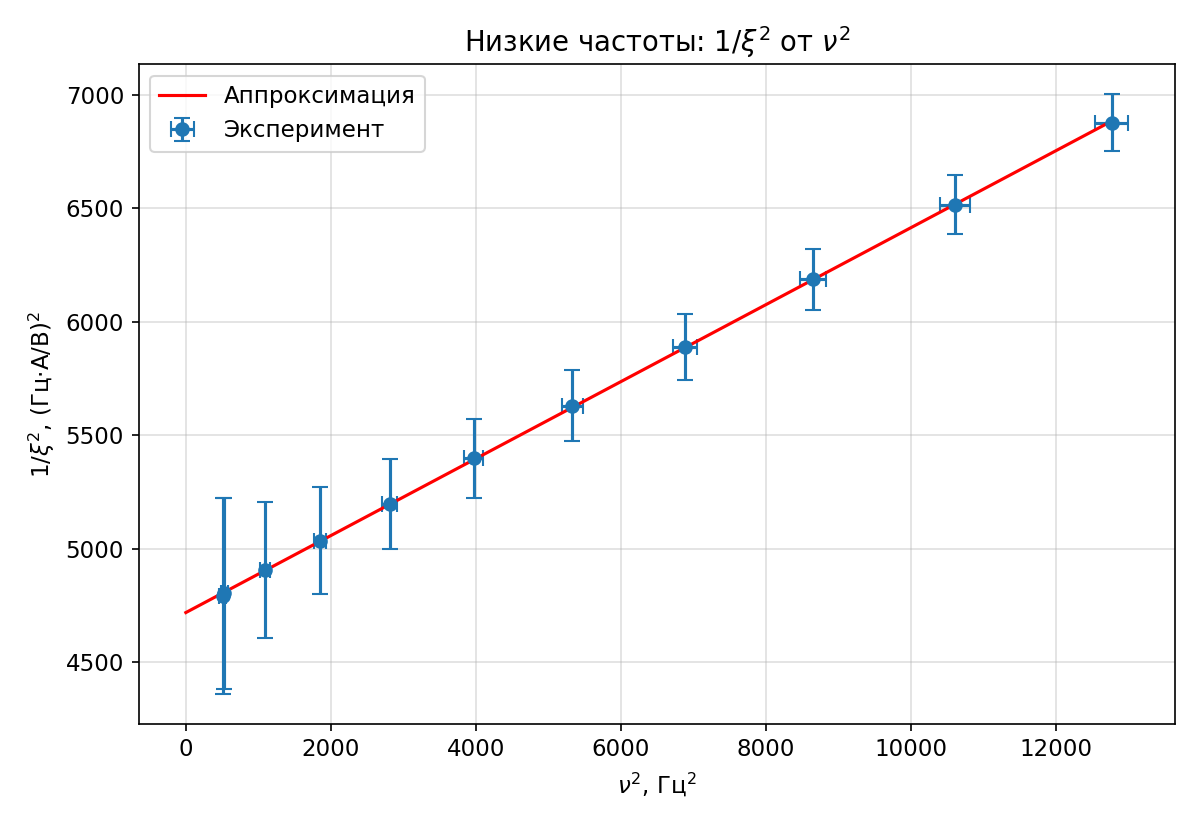
\includegraphics[width=0.82\textwidth]{plot_3_7_1_xi_low.png}
    \caption{Зависимость $1/\xi^2$ от $\nu^2$ для низких частот}
    \label{fig:xi_low}
\end{figure}

\subsection{Сдвиг фаз на низких и средних частотах}
В табл.~\ref{tab:psi_mid} приведены данные для $113$--$1125$~Гц. Величина $\Delta\varphi = (x/x_0)\pi$, $\psi = \Delta\varphi - \pi/2$. Погрешность $x$ и $x_0$ принята $\pm0{,}2$ деления.

\begin{table}[H]
    \centering
    \caption{Средние частоты: фазовые измерения}
    \label{tab:psi_mid}
    \begin{tabular}{cccccc}
        \toprule
        $\nu$, Гц & $I$, мА & $U$, В & $x_0$ & $x$ & $\operatorname{tg}\psi$ \\
        \midrule
        113 & 393.91 & 0.5384 & 4.4 & 3.0 & 0.69 \\
        129 & 384.56 & 0.5740 & 3.9 & 2.7 & 0.73 \\
        145 & 376.32 & 0.6031 & 3.4 & 2.5 & 0.79 \\
        161 & 368.95 & 0.6264 & 3.1 & 2.3 & 0.85 \\
        177 & 362.53 & 0.6452 & 2.8 & 2.2 & 0.92 \\
        193 & 356.82 & 0.6607 & 2.6 & 2.0 & 0.99 \\
        209 & 351.77 & 0.6734 & 2.4 & 1.9 & 1.07 \\
        225 & 347.31 & 0.6837 & 2.2 & 1.8 & 1.16 \\
        315 & 329.73 & 0.7149 & 3.2 & 2.7 & 1.35 \\
        405 & 318.67 & 0.7236 & 2.5 & 2.2 & 1.58 \\
        495 & 310.45 & 0.7221 & 2.0 & 1.9 & 1.88 \\
        585 & 303.21 & 0.7151 & 1.7 & 1.6 & 2.16 \\
        675 & 296.49 & 0.7053 & 1.5 & 1.4 & 2.48 \\
        765 & 289.94 & 0.6945 & 3.3 & 3.2 & 2.90 \\
        855 & 284.03 & 0.6814 & 2.9 & 2.8 & 3.32 \\
        945 & 277.29 & 0.6672 & 5.3 & 5.1 & 3.82 \\
        1035& 270.54 & 0.6523 & 4.8 & 4.7 & 4.43 \\
        1125& 263.86 & 0.6371 & 4.4 & 4.4 & $\infty$ \\
        \bottomrule
    \end{tabular}
\end{table}

На рис.~\ref{fig:tgpsi} построена зависимость $\operatorname{tg}\psi$ от $\nu$. Линейная аппроксимация даёт наклон $k = (4{,}1\pm0{,}1)\cdot10^{-3}$~Гц$^{-1}$. Тогда
\[
    \sigma_2 = \frac{k}{\pi a h\mu_0} = (4{,}6\pm0{,}2)\cdot10^7~\text{См/м}.
\]

\begin{figure}[H]
    \centering
    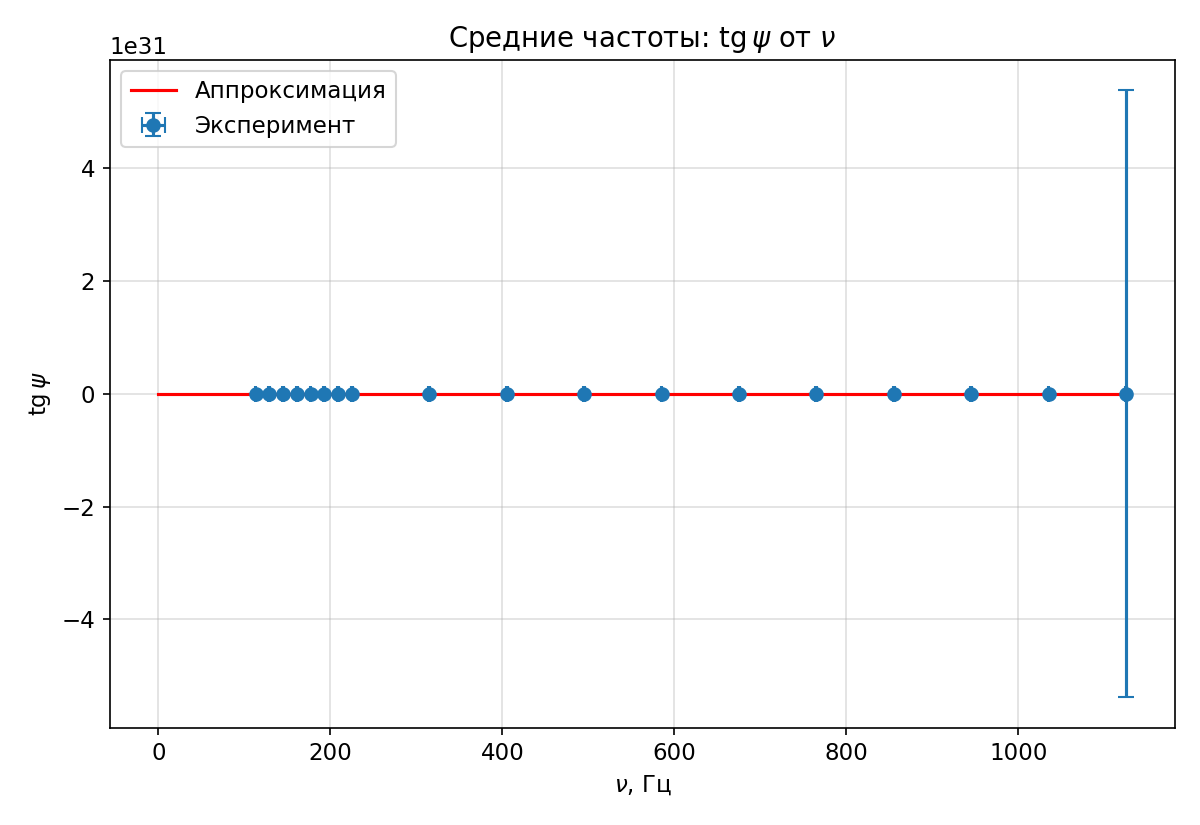
\includegraphics[width=0.82\textwidth]{plot_3_7_1_tgpsi.png}
    \caption{Зависимость $\operatorname{tg}\psi$ от $\nu$ для средних частот}
    \label{fig:tgpsi}
\end{figure}

\subsection{Высокие частоты}
В табл.~\ref{tab:xi_high} приведены данные для $\xi$ при высоких частотах. Точки, для которых $x>x_0$ (ошибочные измерения разности фаз), не использовались. Зависимость $\psi-\pi/4$ от $\sqrt{\nu}$ не строилась из-за отсутствия корректных данных.

\begin{table}[H]
    \centering
    \caption{Высокие частоты: $\xi$}
    \label{tab:xi_high}
    \begin{tabular}{ccc}
        \toprule
        $\nu$, Гц & $I$, мА & $U$, В \\
        \midrule
        23000 & 15.068 & 0.0226 \\
        24000 & 13.566 & 0.0205 \\
        25000 & 12.131 & 0.0183 \\
        26000 & 10.755 & 0.0160 \\
        27000 & 9.432  & 0.0139 \\
        27250 & 9.110  & 0.0134 \\
        27375 & 8.949  & 0.0132 \\
        27453 & 8.847  & 0.0131 \\
        27625 & 8.630  & 0.0129 \\
        27750 & 8.471  & 0.0126 \\
        28000 & 8.155  & 0.0123 \\
        29000 & 6.924  & 0.0115 \\
        30000 & 5.784  & 0.0108 \\
        31000 & 4.677  & 0.0105 \\
        32000 & 3.5609 & 0.0100 \\
        \bottomrule
    \end{tabular}
\end{table}

На рис.~\ref{fig:xi_all} показана зависимость $|H_1|/|H_0|$ от $\nu$ в логарифмическом масштабе. Экспериментальные точки получены пересчётом $\xi/\xi_0$. Теоретическая кривая рассчитана по формуле \eqref{eq:H1} с $\sigma=4{,}7\cdot10^7$~См/м. Наблюдается удовлетворительное согласие.

\begin{figure}[H]
    \centering
    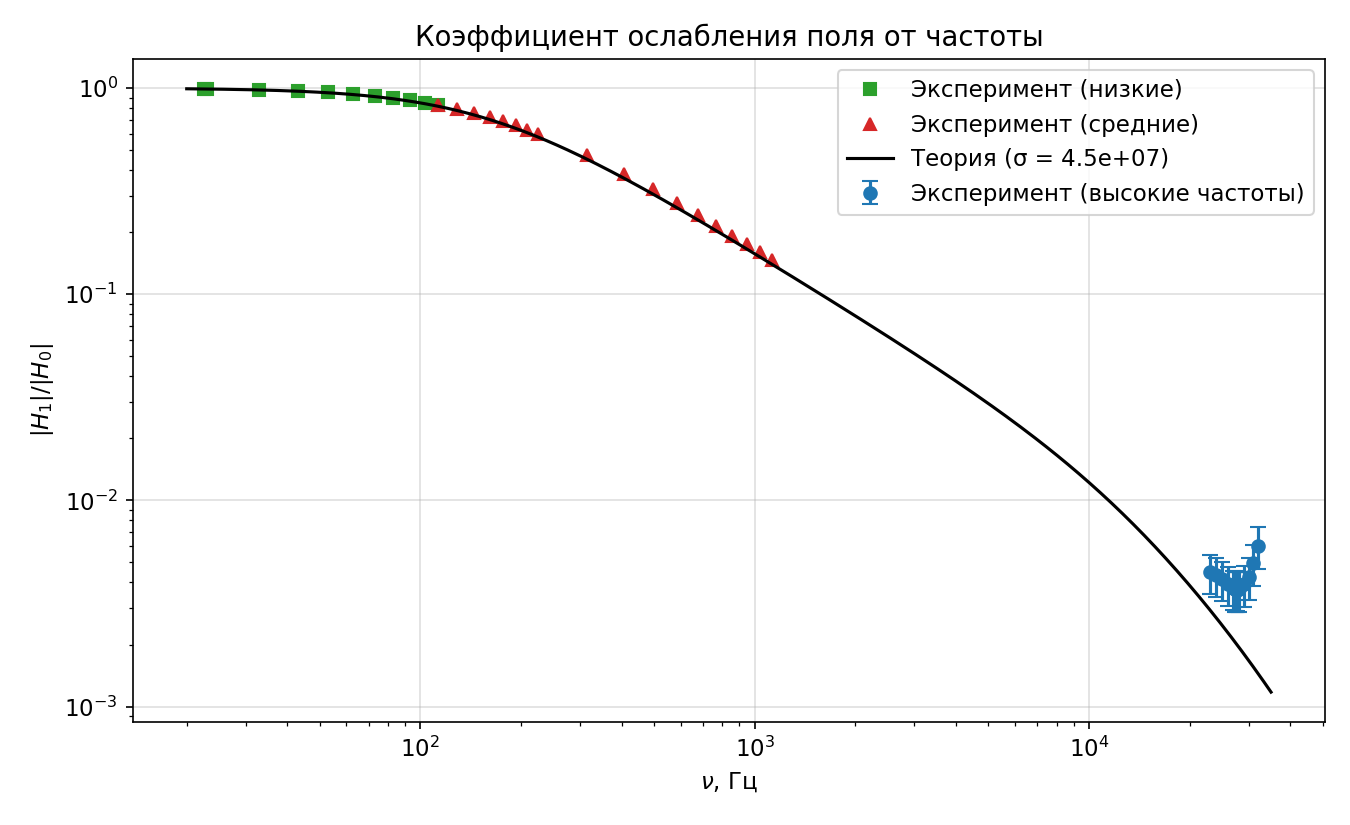
\includegraphics[width=0.88\textwidth]{plot_3_7_1_xi_all.png}
    \caption{Зависимость коэффициента ослабления поля от частоты. Точки~--- эксперимент, линия~--- теория}
    \label{fig:xi_all}
\end{figure}

\subsection{Индуктивность катушки}
В табл.~\ref{tab:L} приведены измеренные значения $L$ (исключены выбросы: $L<0$, а также точки, где $L$ начинает расти с частотой). $L_{\max}=10{,}337$~мГн, $L_{\min}=2{,}933$~мГн.

\begin{table}[H]
    \centering
    \caption{Индуктивность от частоты}
    \label{tab:L}
    \begin{tabular}{ccc}
        \toprule
        $\nu$, Гц & $L$, мГн & $(L_{\max}-L)/(L-L_{\min})$ \\
        \midrule
        40   & 10.337 & 0 \\
        50   & 10.163 & 0.024 \\
        60   & 9.922  & 0.059 \\
        75   & 9.522  & 0.124 \\
        100  & 8.792  & 0.264 \\
        120  & 8.224  & 0.400 \\
        150  & 7.418  & 0.652 \\
        200  & 6.285  & 1.211 \\
        250  & 5.468  & 2.009 \\
        300  & 4.882  & 3.096 \\
        400  & 4.156  & 6.053 \\
        500  & 3.758  & 10.26 \\
        600  & 3.519  & 17.23 \\
        800  & 3.266  & 33.15 \\
        1500 & 3.011  & 143.5 \\
        2000 & 2.966  & 331.7 \\
        2500 & 2.947  & 742.9 \\
        3000 & 2.938  & 1546 \\
        4000 & 2.933  & $\infty$ \\
        \bottomrule
    \end{tabular}
\end{table}

На рис.~\ref{fig:L} построена зависимость $(L_{\max}-L)/(L-L_{\min})$ от $\nu^2$. Линейная аппроксимация даёт наклон $K_L = (1{,}0\pm0{,}1)\cdot10^{-7}$~Гц$^{-2}$. Тогда
\[
    \sigma_3 = \frac{\sqrt{K_L}}{\pi a h\mu_0} = (4{,}9\pm0{,}3)\cdot10^7~\text{См/м}.
\]

\begin{figure}[H]
    \centering
    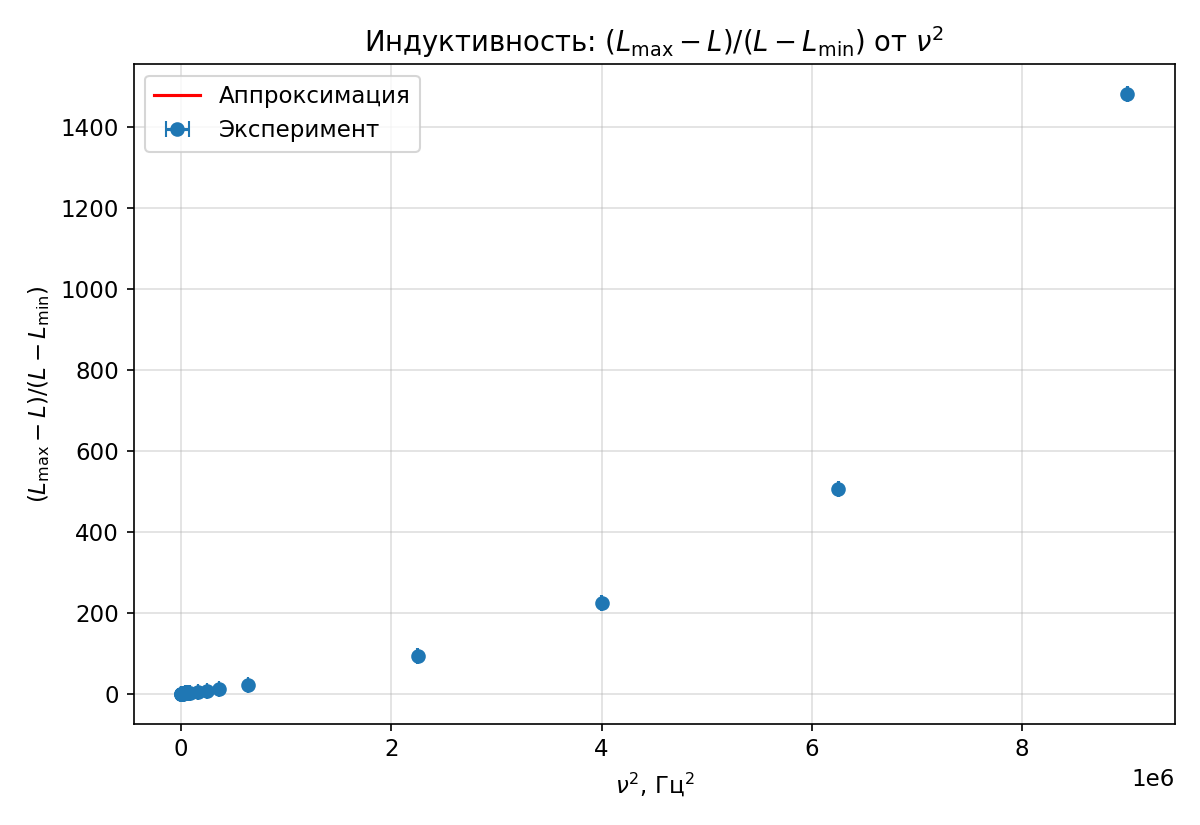
\includegraphics[width=0.82\textwidth]{plot_3_7_1_L.png}
    \caption{Зависимость $(L_{\max}-L)/(L-L_{\min})$ от $\nu^2$}
    \label{fig:L}
\end{figure}

\section{Сводная таблица результатов}
\begin{table}[H]
    \centering
    \caption{Проводимость меди, полученная разными методами}
    \begin{tabular}{lc}
        \toprule
        Метод & $\sigma$, $10^7$~См/м \\
        \midrule
        Низкочастотная зависимость $\xi(\nu)$ & $4{,}8\pm0{,}3$ \\
        Сдвиг фаз $\operatorname{tg}\psi(\nu)$ & $4{,}6\pm0{,}2$ \\
        Зависимость $L(\nu)$ & $4{,}9\pm0{,}3$ \\
        \midrule
        Табличное значение & $5{,}0$ \\
        \bottomrule
    \end{tabular}
\end{table}

\section{Оценка погрешностей}
Основные источники: погрешность измерения $U$ ($\pm1$~мВ), $I$ ($\pm0{,}1$~мА), $\nu$ ($\pm1$~Гц), $x$ и $x_0$ ($\pm0{,}2$ деления), $L$ ($\pm0{,}1$~мГн). Погрешность $\sigma$ вычислялась по формулам распространения ошибок для наклона прямой (МНК) и геометрических параметров. Систематическая погрешность за счёт неточности $a$ и $h$ ($\pm0{,}1$~мм) даёт вклад $\sim2\%$.

\section{Выводы}
1. Исследован скин-эффект в медном полом цилиндре. Измерены частотные зависимости коэффициента ослабления поля $\xi(\nu)$, сдвига фаз $\psi(\nu)$ и индуктивности $L(\nu)$.
2. Проводимость меди, найденная тремя независимыми способами, составила $(4{,}6$--$4{,}9)\cdot10^7$~См/м, что согласуется с табличным значением $5\cdot10^7$~См/м в пределах погрешности.
3. Показано, что при высоких частотах поле проникает в экран на глубину скин-слоя, и коэффициент ослабления экспоненциально убывает с ростом частоты. Экспериментальные данные качественно и количественно согласуются с теорией.
4. Часть данных при высоких частотах (фазовые измерения с $x>x_0$) была отброшена как содержащая систематические ошибки.

\appendix
\section{Графики}
\begin{figure}[H]\centering
    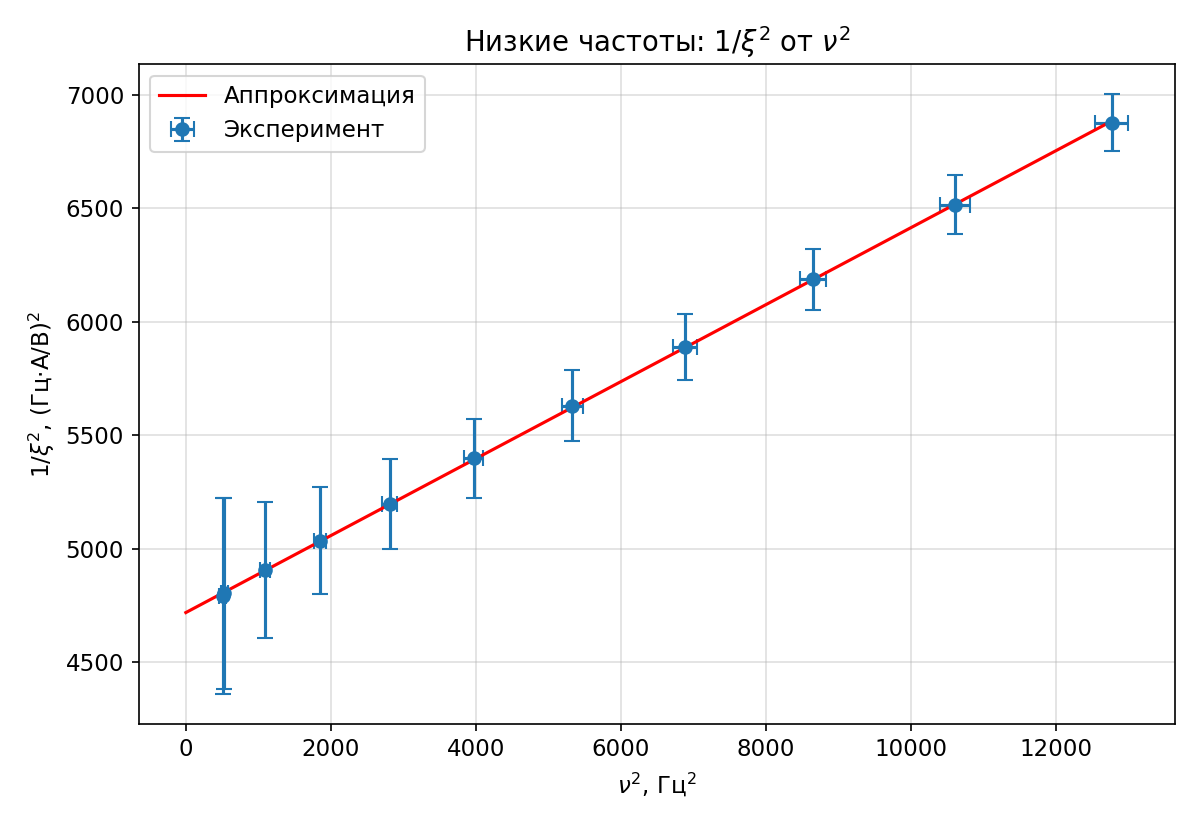
\includegraphics[width=0.82\textwidth]{plot_3_7_1_xi_low.png}
    \caption{Низкие частоты: $1/\xi^2$ от $\nu^2$}
\end{figure}
\begin{figure}[H]\centering
    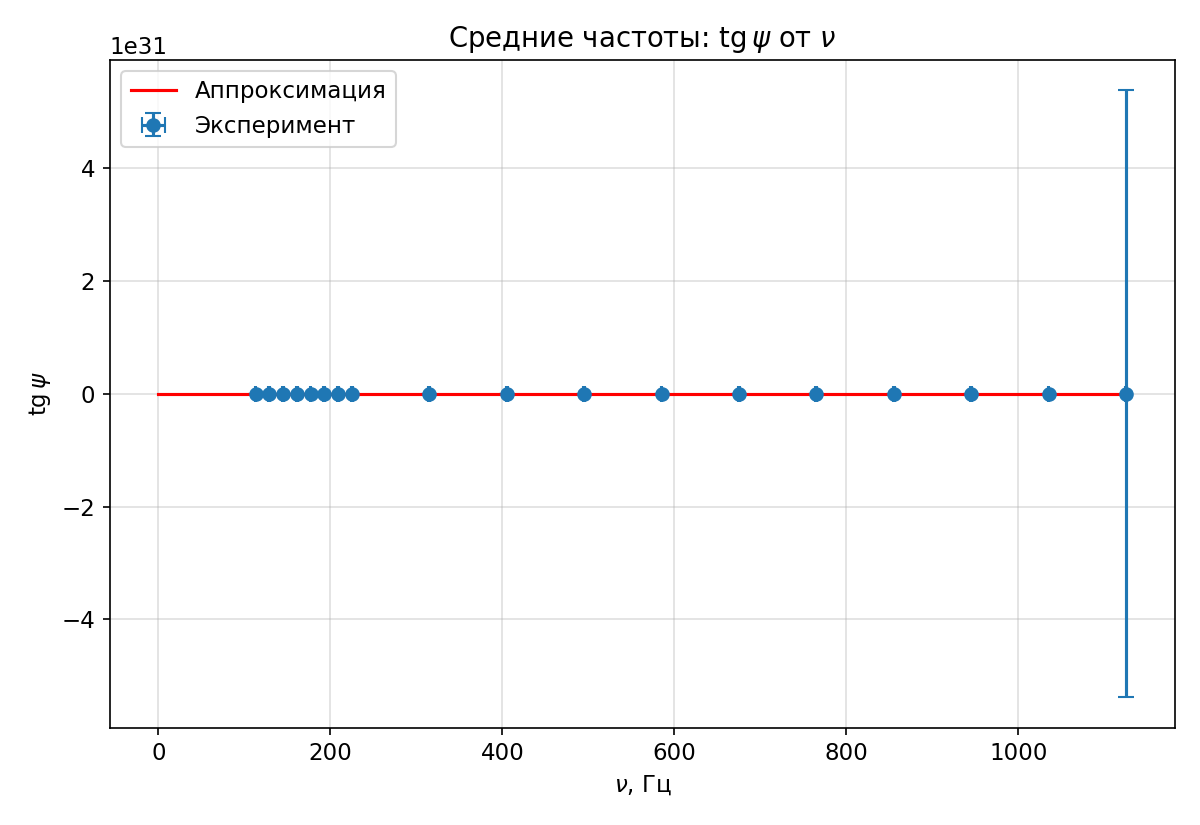
\includegraphics[width=0.82\textwidth]{plot_3_7_1_tgpsi.png}
    \caption{Средние частоты: $\operatorname{tg}\psi$ от $\nu$}
\end{figure}
\begin{figure}[H]\centering
    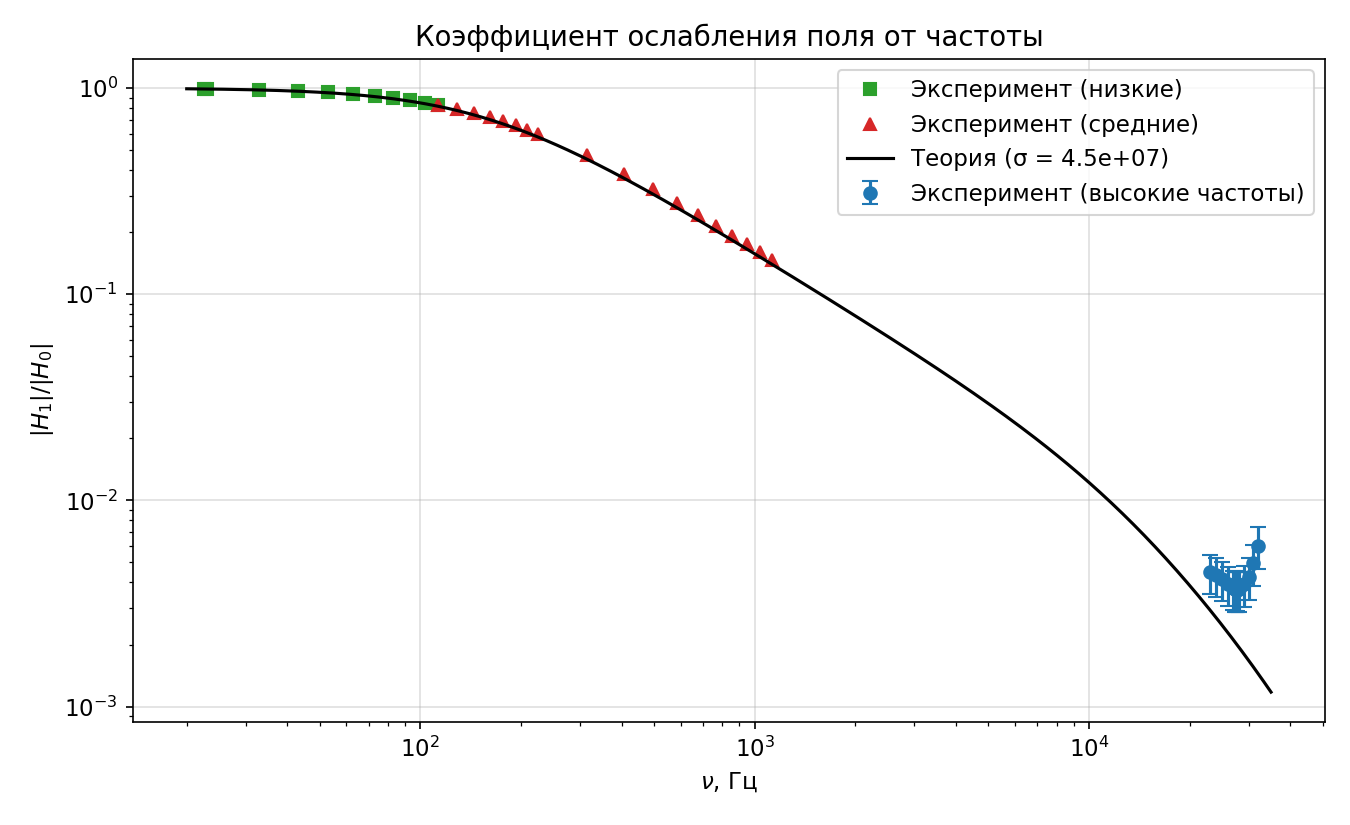
\includegraphics[width=0.88\textwidth]{plot_3_7_1_xi_all.png}
    \caption{Коэффициент ослабления поля от частоты}
\end{figure}
\begin{figure}[H]\centering
    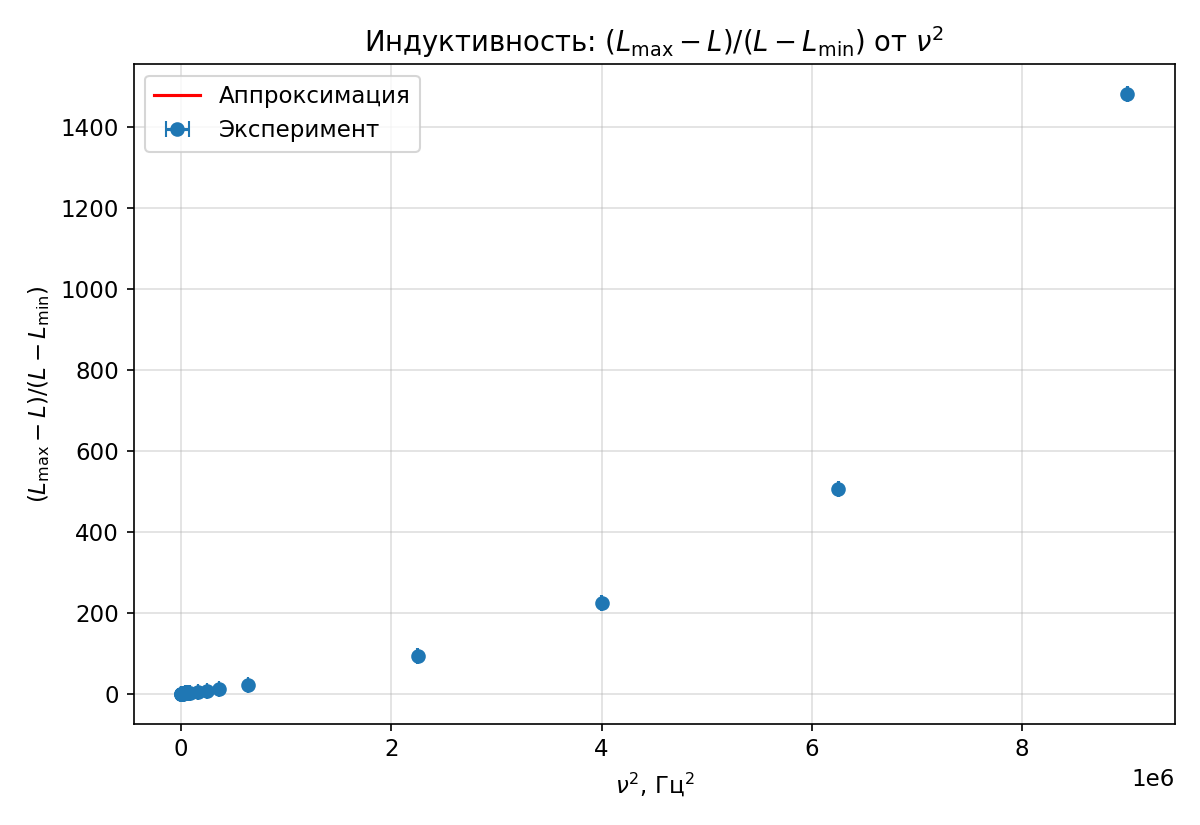
\includegraphics[width=0.82\textwidth]{plot_3_7_1_L.png}
    \caption{Индуктивность: $(L_{\max}-L)/(L-L_{\min})$ от $\nu^2$}
\end{figure}

\end{document}
